\documentclass[11pt, letterpaper]{article}
\usepackage{marvosym}
\usepackage{float}
\usepackage{setspace}
\usepackage{longtable}
\usepackage{caption}
\usepackage{pdflscape}
\usepackage{graphicx}
% DOCUMENT LAYOUT
% \usepackage{geometry} 
\usepackage[margin=1.0in]{geometry}
\usepackage{lineno}
\usepackage[usenames,dvipsnames]{xcolor}
\definecolor{myorange}{RGB}{240, 96, 0}
\newcommand{\mt}[1]{{\textcolor{myorange} {({\tiny MT:} #1)}}}
% \geometry{letterpaper, textwidth=5.5in, textheight=8.5in, marginparsep=7pt, marginparwidth=.6in}
% \setlength\parindent{0in}

\definecolor{linenocolor}{gray}{0.6}
\renewcommand\thelinenumber{\color{linenocolor}\arabic{linenumber}}
% \calclayout %centers text on page.

\usepackage{amsmath}
\usepackage{mathspec}
% \setallmainfonts(Digits,Latin){STIX Two Text}
% \setallmainfonts(Digits,Latin){Baskerville}
% \setallmainfonts(Digits,Latin){Plantagenet Cherokee}
\setallmainfonts(Digits,Latin){Palatino}
% \setallmainfonts(Digits,Latin){Hoefler Text}


% HEADINGS
% \usepackage{sectsty} 
% \usepackage[normalem]{ulem} 
% \sectionfont{\upshape\Large}
% \subsectionfont{\scshape\normalsize} 
% \subsubsectionfont{\upshape\large} 

% PDF SETUP
% ---- FILL IN HERE THE DOC TITLE AND AUTHOR
\usepackage[%dvipdfm, 
bookmarks, colorlinks, breaklinks, 
% ---- FILL IN HERE THE TITLE AND AUTHOR
	pdftitle={Many claims of group polarization are plausibly false due to inappropriate
    statistics},
	pdfauthor={Matthew A. Turner},
	pdfproducer={https://mt.digital}
]{hyperref}  
\hypersetup{linkcolor=blue,citecolor=blue,filecolor=black,urlcolor=MidnightBlue} 

\usepackage{apacite}
\usepackage{booktabs}
\usepackage{authblk}

\newcommand{\sigmapre}{\sigma_\mathrm{pre}}
\newcommand{\sigmapost}{\sigma_\mathrm{post}}

\newcommand{\normalpre}{\mathcal{N}(\mu, \sigmapre)}
\newcommand{\normalpost}{\mathcal{N}(\mu, \sigmapost)}

\newcommand{\ordmeanpre}{\langle o_{\mathrm{pre}}}
\newcommand{\ordmeanpost}{\langle o_{\mathrm{post}}}

\begin{document}

\title{Many claims of group polarization are plausibly false due to inappropriate
    statistics}
% \shorttitle{Group polarization or simple consensus?}
% \author[1,2]{{Matthew A.~Turner}}
\author[1]{{Matthew A.~Turner}}
% \affil[1]{Department of Earth System Science, Stanford University}
\affil[1]{Division of Social Sciences, Stanford Doerr School of Sustainability, Stanford University}

% \author[3,4,5]{{Paul E.~Smaldino}}
\author[2,3]{{Paul E.~Smaldino}}
\affil[2]{Cognitive and Information Sciences, University of California, Merced}
% \affil[4]{Center for Advanced Study in the Behavioral Sciences, Stanford University}
\affil[3]{Santa Fe Institute}



\maketitle
% \setlength{\parindent}{15pt}
% \maketitle

\spacing{1.5}

\linenumbers
% \modulolinenumbers[3]

\begin{abstract}
  \noindent
  % Psychology is beset by three crises: the reproducibility crisis, the
  % generalizability crisis, and the theory crisis. New verbal theories for various
  % phenomena are constantly being developed orthogonal to other theories, all based on
  % mostly unreproducible analyses; even if a positive result is in some sense ``true''
  % it may not account for all the variance present in a set of observations---studies
  % thus fail to generalize because their results do not account for this variance.
  % There is another related problem: a phenomenon may be ``reproducible'' only
  % because studies of the phenomenon systematically misuse statistics in such a way
  % that induces false positives for each succeeding ``replication.'' 
  \emph{Group polarization} refers to the observation that like-minded novel groups tend to
  become more extreme in their opinions after discussion as group members found consensus.
  \emph{Consensus} here refers to decreasing opinion variance; we further define
  \emph{simple consensus} as a process where group opinion variance decreases but
  the mean opinion does not change.
  Here we show that many published experimental detections of group polarization are explained
  equally rigorously as \emph{simple consensus}. 
  The reports we analyze assumed in their statistical analyses 
  that both latent psychological opinions \emph{and} the ordinal 
  reported opinions (e.g., on a Likert-type scale) are continuous. We use
  a generative model to demonstrate that 95\% of sixty experimental conditions
  across ten foundational group polarization papers report plausibly false detections of
  group polarization. We show that simulated data from these plausibly false
  cases often fools a $t$-test into reporting significant group polarizaiton
  effects, but a Bayesian implementation of the more appropriate ordered-probit
  model reliably identifies these data as
  representing simple consensus, not group polarization.
  Our results demonstrate the need for a new wave of group polarization research
  that uses rigorous statistical methods appropriate for the study design. 
  Our approach can be used beyond group polarization
  research to analyze results from any experimental paradigm that may use statistical models that
  are poorly matched to the study design. Replications are worthless if the statistics are wrong.

  % To show this, we developed a
  % novel generative model that provides two levels of evidence that an historical
  % published empirical finding of group polarization is plausibly false.  Our model
  % can be used to evaluate additional studies in group polarization and beyond, even
  % if the reported data and significant metrics are incompletely reported, and the
  % original raw data has been lost to time.  This may be just the tip of the
  % plausibly-false-positives-in-psychology iceberg, both for group polarization
  % studies and for the legion psychological results that model ordinal observations of
  % opinions, beliefs, emotions, or any other latent psychological variable that is
  % theoretically continuous, but measured using an ordinal scale.  
\end{abstract}
\clearpage

\begin{quote}
In our introductory social psychology course, 
we have for many years used the [group polarization experimental paradigm] as
a laboratory exercise. The exercise works beautifully, but one must be
careful to forewarn a class that [group polarization] does not occur with every 
group\ldots and that the effect is not large. 
\par\raggedleft\cite[p. 205]{Brown1986}
\end{quote}

\begin{quote}
One of the most robust findings in social psychology is that of attitude polarization 
following discussion with like-minded others.
\par\raggedleft\cite[p. 267]{Cooper2001}
\end{quote}

\section{Introduction}

\begin{itemize}
  \item 
    \emph{Group polarization} is a process where the mean opinion of a 
    like-minded group becomes more extreme over time~\cite{Brown1986,Brown2000}. 
    It is therefore an important component process in
    the broader process of increasing political polarization that can hamstring
    governments~\cite{Mason2018UncivilAgreementBook,Klein2020}.
  \item
    Individuals' opinions in group polarization experiments are typically 
    measured using an ordinal scale, such
    as a Likert scale, where behavioral experiment participants' internal, theoretically
    continuous, opinions are converted to one of several opinion bins indiciating
    their degree of agreement or disagreement with some prompt statement.
  \item
    Recently, however, it has been shown that it is critical to use 
    appropriate statistical methods when using experimental designs that 
    measure continuous latent psychological variables with ordinal
    measurements---failure to do so can result in false positive support for
    the presence of experimental effects~\cite{Liddell2018}.
  \item
    In this paper, we develop a generative modeling approach for evaluating whether or
    not published detections of group polarization are plausibly false, i.e.,
    whether they are \emph{plausibly-false positives} (PFPs). 
  \item
    We found significant evidence that many published group polarization findings
    are indeed plausibly false since we found distribution parameters that
    generated simulated pre- and post-discussion data that a $t$-test found
    to be from distributions with different means, although there was no difference
    in mean, only a difference in variance. 
  \item
    Although a $t$-test may be fooled by simple consensus under ordinal measurements,
    we show that a more appropriate ordered probit model of the data yield no
    such plausibly-false positives.
  \item
    Our work shows the need for using appropriate statistical tests, as well as
    the need for a consistent experimental paradigm so that meaningful meta-analyses
    can be performed for theoretical integration and rigorous understanding of
    the group polarization effect, should it prove to occur in future group
    polarization studies that use proper statistics. In addition to avoiding
    $t$-tests, future group polarization studies can be more reliable by
    accounting for random effects arising from, e.g., socioeconomic status,
    gender, and other individual-level factors that may bias how much and in what
    direction a participant changes their opinions. Failure to do so can result 
    in artificially-inflated effect sizes~\cite{Yarkoni2021}.
\end{itemize}

\subsection{Group polarization}

Group polarization is often induced in behavioral experiments by first answering
an opinion prompt, grouping
relatively like-minded individuals together to discuss the prompt, then 
again polling opinions; the change in mean opinion towards a more extreme
consensus than the initial mean is the amount of group polarization that has occurred
(Figure~\ref{fig:groupPolarizationSchematic}). 

While all ten studies scrutinized here use the general experimental procedure
outlined above (Figure~\ref{fig:groupPolarizationSchematic}), each study and constituent 
experimental condition have idosyncracies that makes the results themselves
more opaque, and that makes comparison of different studies' findings more
difficult. (REVIEW A FEW SIMPLE EXAMPLES). A detailed examination of each study's
idiosyncracies is given in Table~\ref{tab:conditionsComparison}.

\begin{figure}
  \caption{Group polarization is experimentally induced by first gathering
  participant responses to an opinion prompt (A). Then groups of like-minded 
  individuals discuss the prompt (B). Group 
  polarization occurs if the mean post-discussion opinion is more extreme 
  than the mean pre-discussion opinion (C).}
  \label{fig:groupPolarizationSchematic}
  \centering
  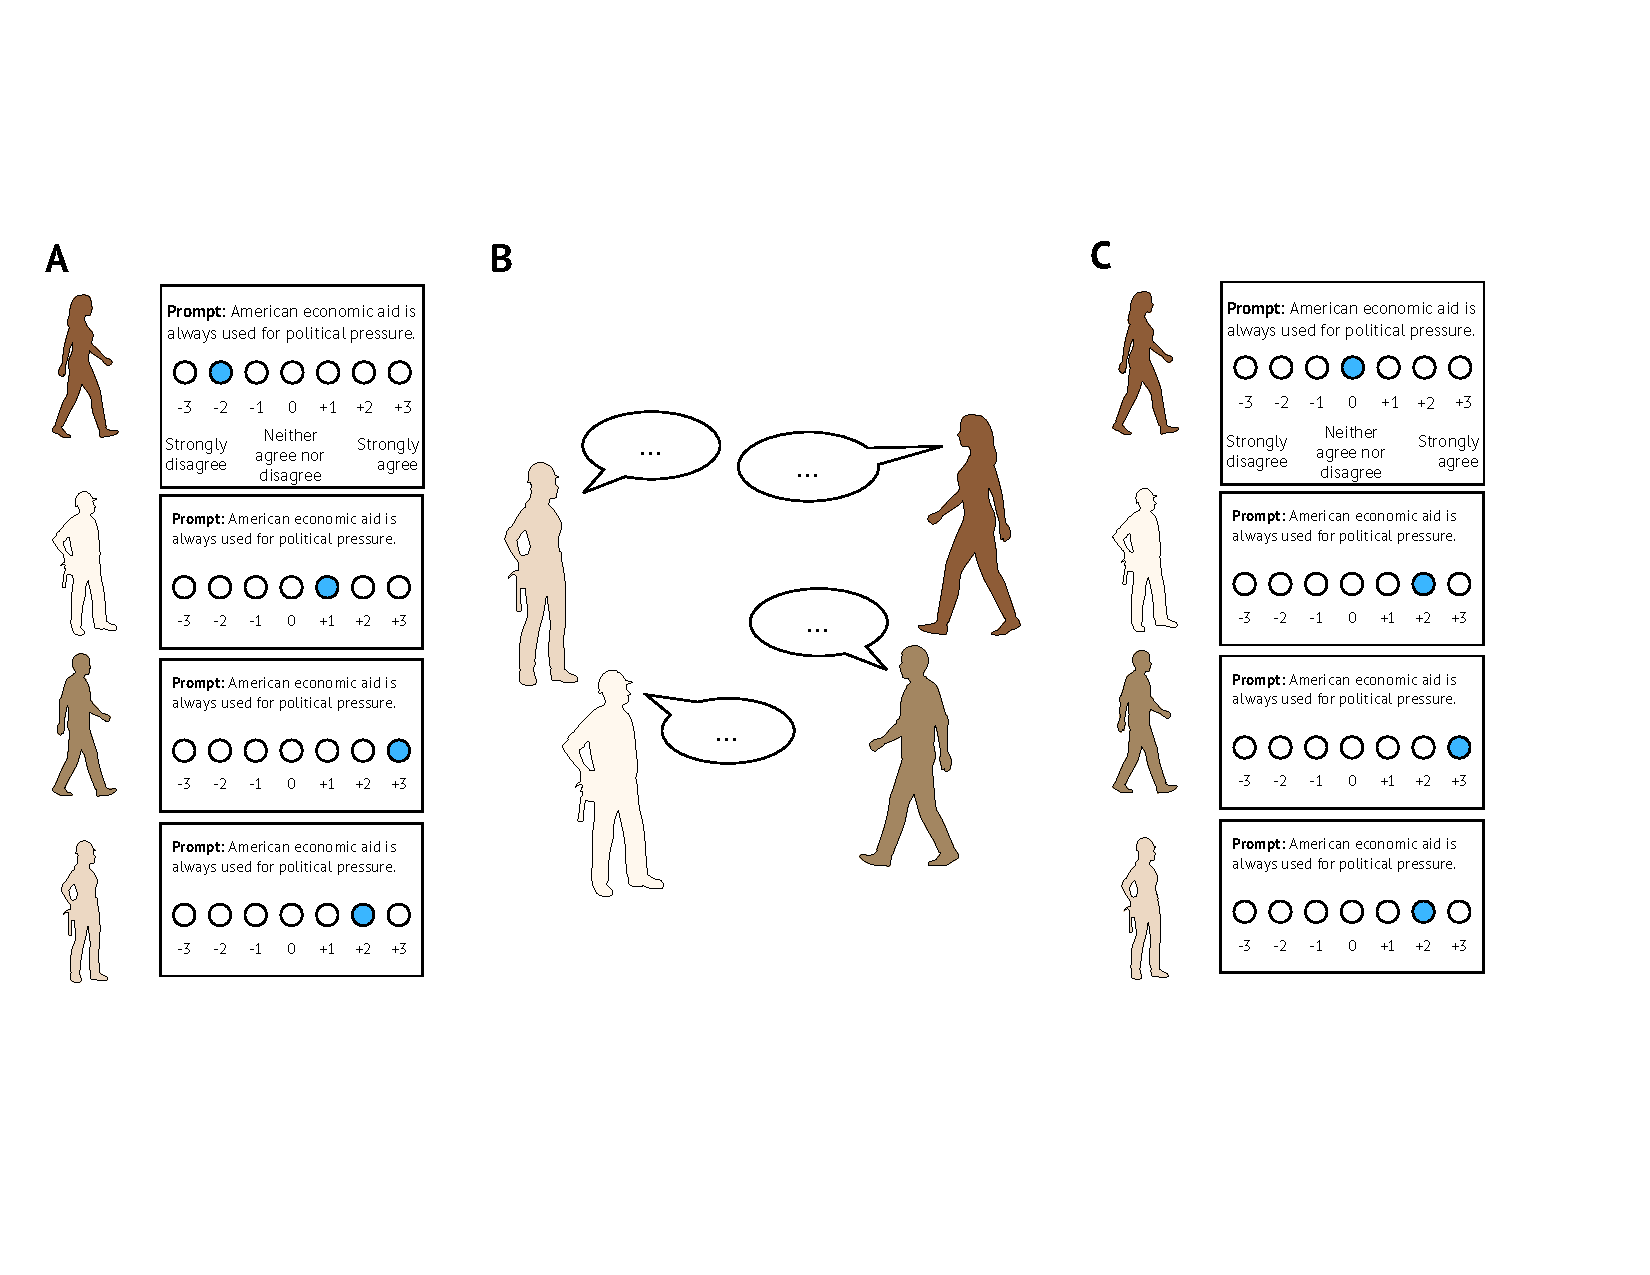
\includegraphics[width=\textwidth]{Figures/GPExperimentSketch.pdf}
\end{figure}



\spacing{1.0}

% \newgeometry{margin=1cm} % modify this if you need even more space
\begin{landscape}


%put your table here

% \begin{table}
%   \small
%   \begin{tabular}{p{1.5in}lp{2.5in}p{3.5in}}
  % \begin{longtable}{p
  \small
  \begin{longtable}{p{1.5in}lp{2.0in}p{4.0in}}
    \caption{Summary of idiosyncracies across experimental conditions in the
    studies we scrutinized for plausibly-false positives.}
    \label{tab:conditionsComparison}\\
  % \begin{longtable}{llll}
  % \begin{tabular}{llll}
  \toprule
  \textbf{Article (Article Tag)} & \textbf{Condition Tag} & \textbf{Prompt} & \textbf{Description} \\
  \midrule
  \citeA{Moscovici1969} (Moscovici1969) & Americans-Opinion & American economic aid is always used for
  political pressure.  & 11 total prompts (1 reported), all 7-point scales. Unclear how data was aggregated. \\
  \midrule
  ~(Moscovici1969) & DeGaulle-Opinion & Charles De Gaulle is too old to (be president) & 12 total prompts (1 reported), all 7-point scales. Unclear how data was aggregated. \\
  \midrule
  ~(Moscovici1969) & DeGaulle-Judgment & Charles De Gaulle is too old to (be president) & Same as
  above, except ``subjects were asked first to judge individually and then to reach consensus as a
  group in evaluating the varoableness or unfavorableness of each item toward de Gaulle,
  regardless of whether they agreed...~with the content of the item.'' \\
  \bottomrule
  \end{longtable}
  % \end{tabular}
% \end{table}

\end{landscape}
\restoregeometry

\spacing{1.5}

\subsection{Statistical inference in opinion change}

2-3 par: the right way; what GP studies do; why it's a problem (N-1 sents) and how
to fix it (1 sent)

When 

\begin{itemize}
  \item 
    Group polarization studies use null-hypothesis testing that implicitly
    assume (1) \emph{opinions} (or other equivalent latent psychological variables
    such as \emph{attitudes} or \emph{beliefs}) are continuously-valued, and
    (2) 
  \item
    The exact null-hypothesis testing procedure varies between studies $t$-tests, ANOVA, etc. 
\end{itemize}

Recently, problems with using have been made clear~\cite{Liddell2018}.
The way to fix this problem going forward is to use a thresholded-normal 
statistical model for group polarization data, or other related statistical 
model that accounts for opinion binning~\cite[Ch. 23]{Liddell2018,KruschkeDBDA}.

\subsection{Study selection and overview}

Studies were selected to be either influential papers, based on citations or
author prominence, that test either examine
group polarization in political opinions, and to be representative of investigations
of four primary group polarization explanations extant in the literature.
At the time of paper selection we did not examine the statistical methods in detail beyond
checking that they indeed used 

Because of the difficulties casting individual research articles into our modeling
framework, and the central task of creating the model and analyzing this first
batch of studies with it, we limit our analysis to 10 studies. It is problem
enough that these 10 prominent studies have the problems we demonstrate they
plausibly do. Problems among these 10 suggest the problem may be more wide spread. 
When we do more analyses
they will be aided by improved data management systems for applying this model to 
additional studies (eventually outside of group polarization).

Statistical problems among these studies are not limited to a mismatch between
measurement and statistical procedures, which requires the detailed treatment
we provide in this paper. Other problems are more pedestrian.
One major issue shared by several studies
is the use of unpaired $t$-tests to detect group polarization. Since the same
group has their opinions measured twice over time, the opinions are correlated
and so a paired $t$-test would be required for test assumptions to be met 
(assuming all other paired $t$-test assumptions were met, 
which of course they are not, which is why our paper here is necessary).
In some cases the reported shifts were ``significant'', 
but not truly ``group polarization'' shifts, i.e., 
shifts from initially biased group opinions
to more extreme group opinions biased in the same direction; instead shifts 
were from a neutral initial group opinion to a biased group opinion 
(as in, e.g.,~\citeA{Abrams1990} Uncategorized2), or from
an opinion biased in one direction (as in, e.g.,~\citeA{Abrams1990} Categorized1,
Categorized2, AND OTHERS???). In some results of \citeA{Freidkin1999a}, 
shift values are reported with their
standard deviations---but the shift standard deviations are greater than the
shifts themselves, indiciating that zero shift is included in the observed
shift confidence interval. This is \emph{prima facie} a negative result that
should not have been counted as evidence of group polarization. 

Some group polarization studies do not measure continuous latent opinions using
a metric scale, and so are not affected by the floor and ceiling effects that
undermine a good number of experimental results, as we examine here. There may,
however, be other problems, such as non-group polarization shifts and the use
of unpaired $t$-tests when paired tests are required.



\subsection{Research overview}

In this paper we analyze whether published statistical detections of group 
polarization obtained through null-hypothesis statistical tests
are plausibly false because they can be explained equally well by simple consensus
where the mean group opinion does not change over time, but opinion variance does.
This analysis requires several preliminary steps. 
First we formally develop our generative model of simple consensus and group 
polarization in terms of changes in group opinion mean and variance from 
pre- to post-deliberation. Then we developed a search algorithm for identifying 
which, if any, simple consensus scenarios with 
constant latent mean and pre- and post-deliberation opinion variances 
could generate published observations of group polarization. To apply this model
and algorithm to published results, we developed an interactive web application
for data input and to test which different potential simple consensus scenarios 
could generate group polarization opinion shifts. After identifying plausibly false
detections of group polarization we examine whether the identified simple
consensus scenario (parameters?) can indeed generate data to fool the 
paper's null-hypothesis tests into thinking the data actually support the inference
that simple consensus did not occur. Finally, we examine whether, in these same
plausibly false detections, a Bayesian thresholded-normal statistical model
will accurately identify simple consensus instead of falsely detecting group
polarization.

\section{Model}

Our model represnts the generative process of finding different forms of group consensus
in group polarization experiments, and the process of measuring that consensus using
an ordinal measurement scale, e.g.\ a Likert-type scale. This model operationalizes two
relevant forms of consensus: \emph{simple consensus} and \emph{group polarization}.
\mt{Need to explain in Intro why consensus should occur along with group
polarization} 
% Group polarization experiments are designed to result group consensus
% since they group together like-minded individuals to see if they become more
% extreme after discussion~\cite{Turner2018}.

We collected group polarization data from ten empirical studies with sixty constituent
experimental conditions across all studies. We recorded the reported opinion shift and pre- and
post-deliberation mean opinions, and the number of participants
in each condition, as long as this data was available---\citeA{Burnstein1975} 
did not report pre- and post-deliberation
means, only the shift in means. We did not include experimental treatments that did not 
yield a positive detection of group polarization since we are only estimating
the rate of plausible false positive detections of group polarization. 

Based on this data

% In two cases, reported opinion and shift values were converted from an ordinal
% scale to a percentage scale, specifically \citeA{Friedkin1999a} and \citeA{Krizan2007}.
% The authors in these papers did report the original ordinal measurement scale,
% so we converted the means back to the orignial measurement scale.
% In a few cases from \citeA{Friedkin1999a} we did not need to apply our 
% model to the reported data because we could determine a reported opinion shift was 
% \emph{prima facie} false since reported opinion shift magnitudes
% were smaller than the standard deviation in shifts (see Table 1, p. 868, \emph{ibid}),
% despite Friedkin's claim that regressions (not clearly defined) on all shifts 
% yielded $p < 0.05$~\cite{Kruschke2018c}.


\subsection{Latent opinions, ordinal measurements, and how simple consensus can look like
group polarization}


We begin by developing a formal model of ordinal measurement of latent continuous
opinions (model variables and parameters are given in Table~\ref{tab:modelVariables}).
First, we assume that participant $i$ has latent opinion at time $t$ that is drawn from
a group-level normal distribution,
\begin{equation}
  o_{i,t} \sim p(o; \mu_t, \sigma_t) = \mathcal{N}(\mu_t, \sigma_t).
  \label{eq:opinionDistribution}
\end{equation}
\noindent 
This distribution has mean $\mu_t$ and standard deviation $\sigma_t$.
This form is chosen to
reflect the common statistical analysis used by group polarization studies,
not because it is statistically appropriate---in fact it is not, which is what
we aim to show in this paper.

It is appropriate to assume opinions are normally distributed because published
group polarization studies use some sort of $t$-tests, or similar tests, which are designed
to detect whether the mean of two distributions are the same or not. This imposes the
implicit assumption that opinions themselves are normal. But as we will show, 
metric statistical tests such as $t$-tests reliably generate false rejections
of the null hypothesis that there is no difference between two distributions' means.

\subsubsection{How simple consensus can look like group polarization}

Simple consensus can look like group polarization when (1) the mean latent opinion
does not change; (2) both more and less extreme opinions move toward this 
unchanged latent mean (i.e., opinion variance shrinks due to consensus); 
and (3) an ordinal scale is used that bins all extreme
latent opinions into the same extreme bin even though those means have changed,
but opinion bins that are less extreme or of opposite polarity more accurately
reflect the underlying change in latent opinion distribution. This process is
illustrated in Figure~\ref{fig:consensusDistroIllustration}, where we show
a toy example of what can occur when the pre-consensus
opinions (upper left plot) 

\begin{table}[h]
  \caption{Variables used in the formal model of group polarization from simple consensus.}
  \label{tab:modelVariables}
  \begin{tabular}{cp{5.0in}} \toprule
   Symbol & Description  \\ \midrule  
   $t \in \{\mathrm{pre}, \mathrm{post}\}$ & Time, either \emph{pre}- or
                                           \emph{post}-discussion \\
   $\mu$  &   Latent mean, assumed constant for simple consensus \\ 
   $\sigma_t$ & Latent standard deviation at time $t$ \\
   $p(o;\mu,\sigma_t)$ & Normal latent distribution of opinions with mean
                         $\mu$ and variance $\sigma_t^2$ \\
   $k \in \{0,\ldots,K\} $ & Threshold index ($k$) between 0 and total number of
         ordinal bins, $K$ \\
   $b_k$ & Opinion bin $k$; note there is no $k=0$ bin. \\
   $\theta_{k-1},~\theta_k$  & Lower, upper threshold value for binning latent opinions into
     bin $b_k$ \\
   $p(o \in b_k; \mu, \sigma_t)$ & Ordinal density of binned opinions in bin $b_k$ 
            (Equation~\ref{eq:binFrequency}) \\
   $\langle o_t \rangle$  &   Observed mean opinion calculated from ordinal data at time $t$ \\
   \bottomrule
  \end{tabular} 
\end{table}

\begin{figure}
  \caption{\emph{Simple consensus} occurs in a group when its latent opinion
  distribution variance decreases, but the mean does not change (A). When 
latent opinions are measured on an ordinal scale, the mean of the distribution
can be distorted by ceiling (or floor) effects (B). Group polarization 
can appear to have occurred where the mean of the observed opinions appears
to increase despite the latent mean being constant (C).}
  \label{fig:consensusDistroIllustration}
  \vspace{1em}
  \centering
    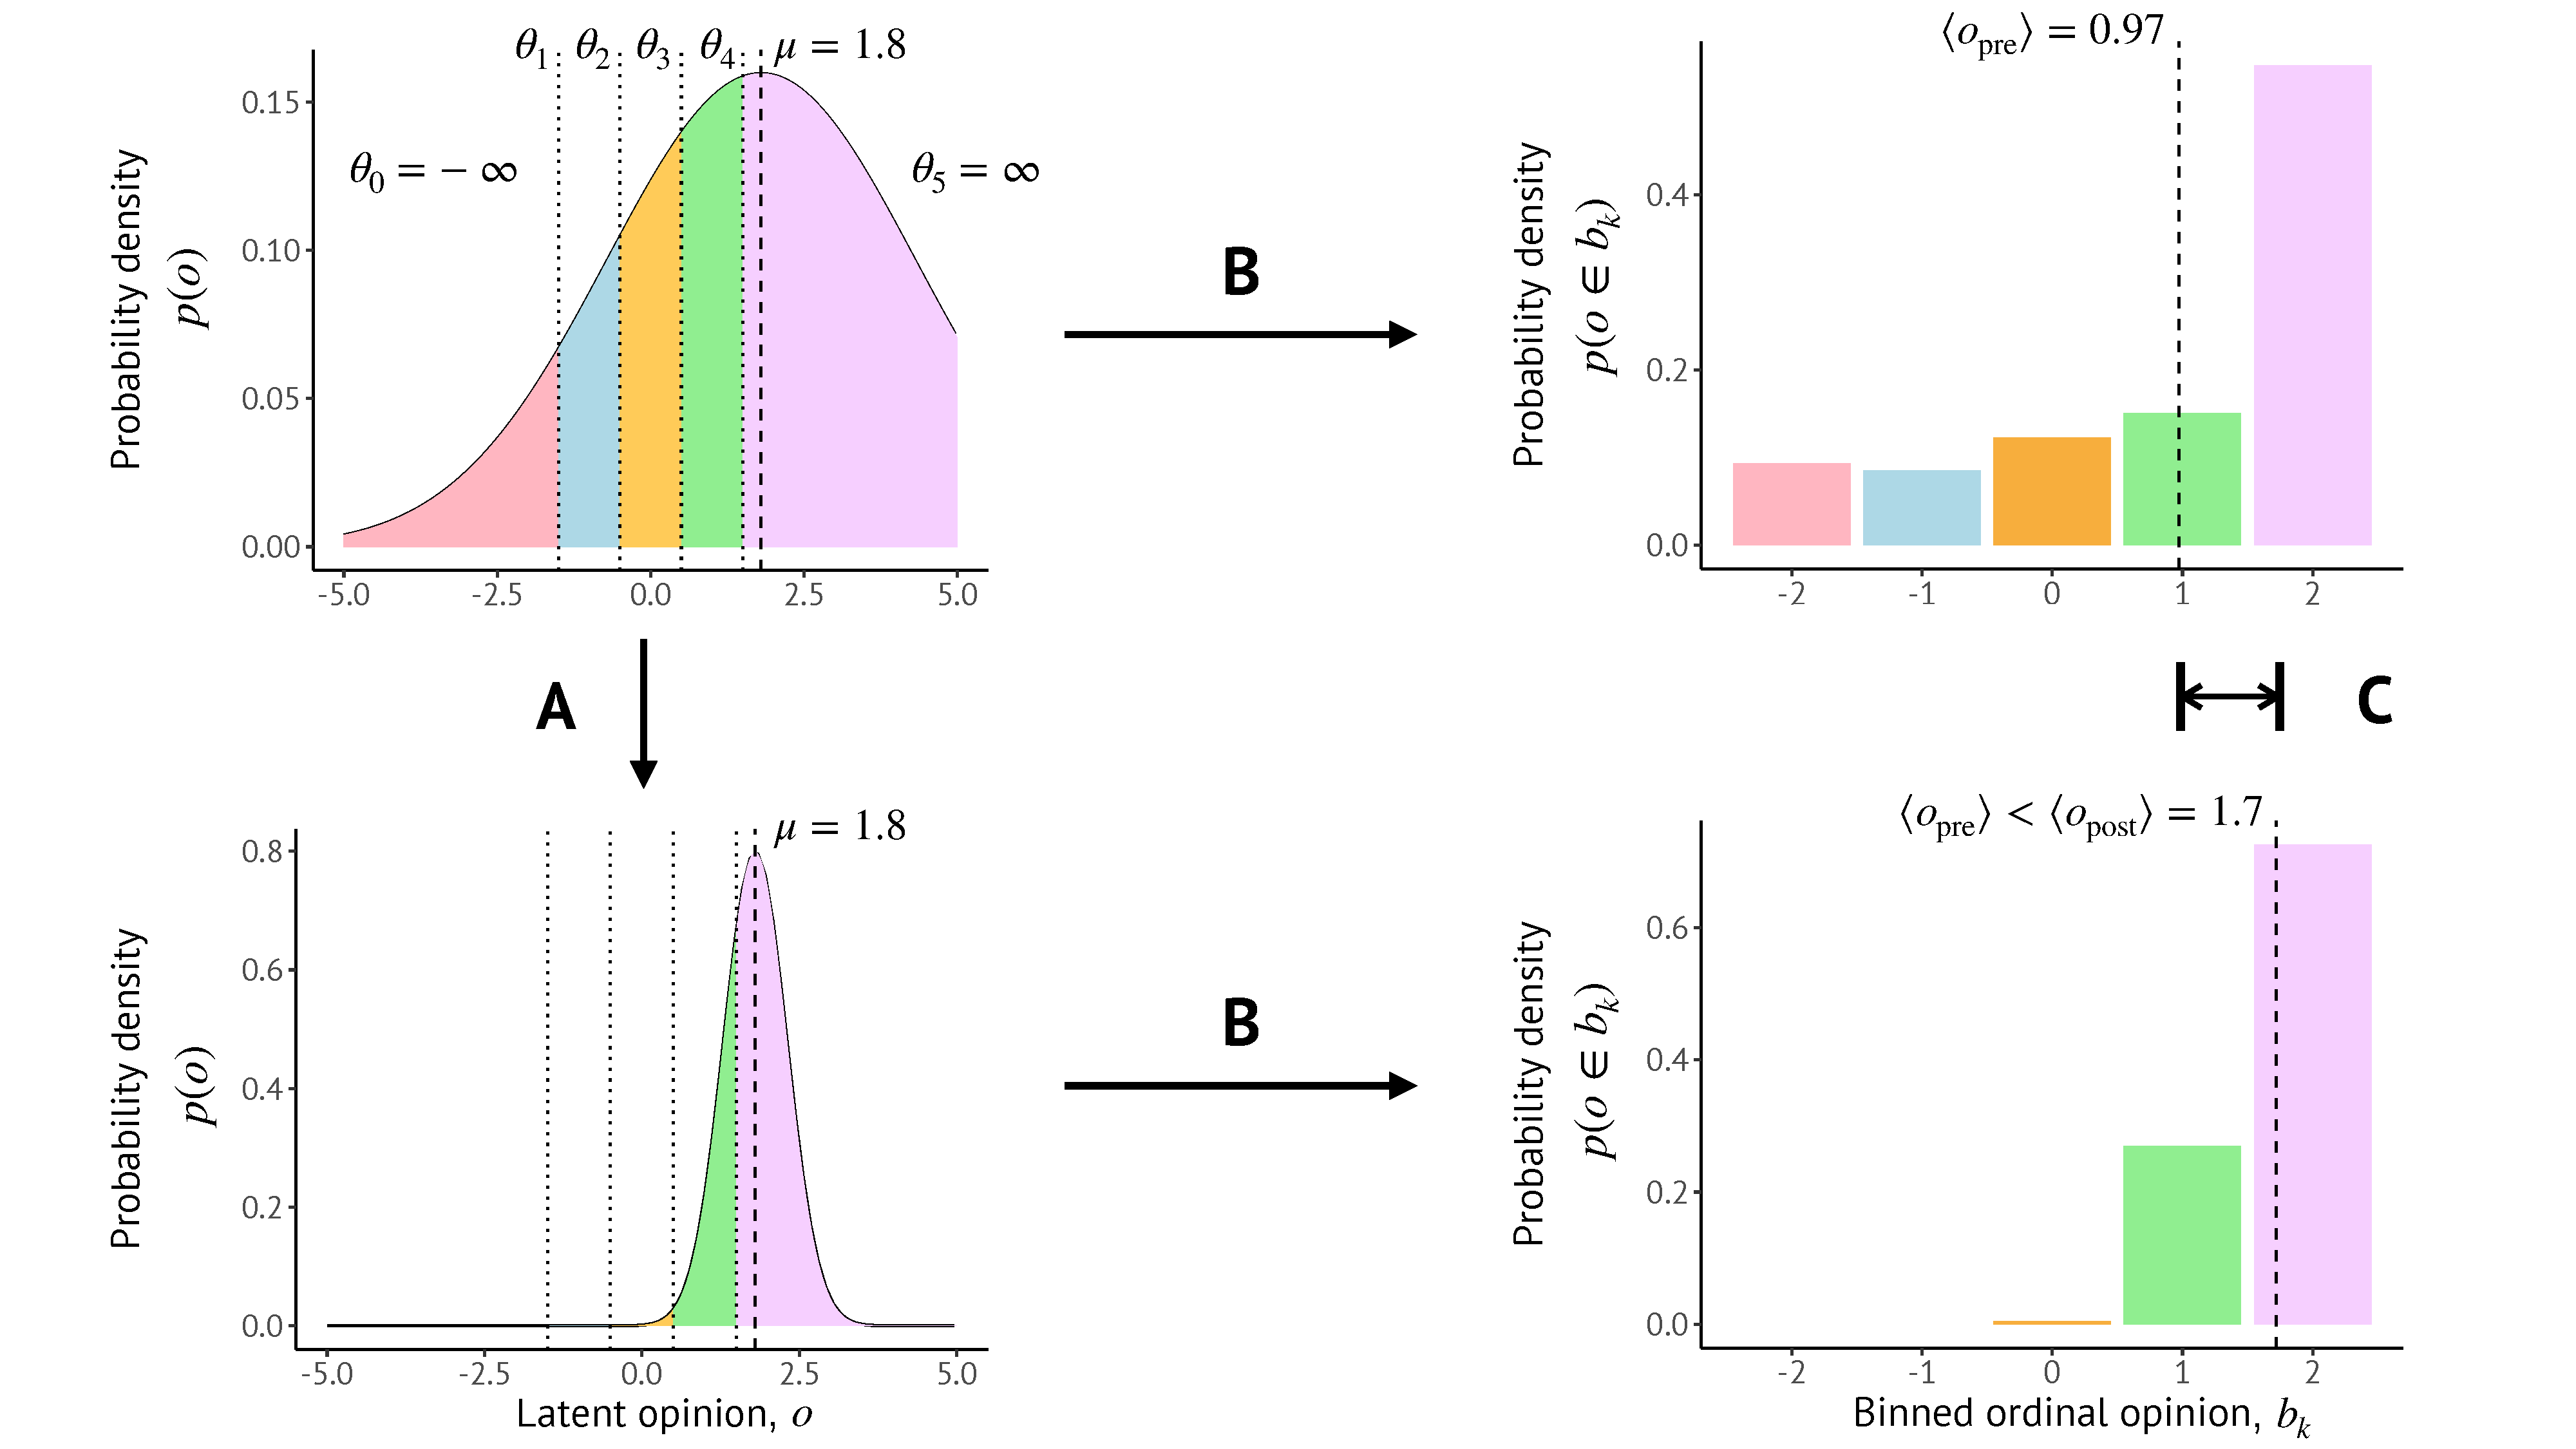
\includegraphics[width=1.0\textwidth]{ConsensusDistroIllustration/figure.pdf}
\end{figure}

This distributional view models the measurement of $N \to \infty$ participant opinions,
which results in a histogram of frequency of opinions
in each bin, i.e., $o_{i,t} = b_k$. The frequency of responses in each bin is 
the integral over the continuous normal probability density function from 
one bin threshold to another. This transforms the probability density 
function from $p(o_{i,t};~\mu_t, \sigma_t)$ to the probability
of observing a reported opinion of each bin value. 
The probability of observing an opinion in bin
$b_k$ is calculated by integrating the normal probability density 
function over the range of $\theta_{k-1}$ to $\theta_{k}$. 
Formally, we write the 
probability of observing an opinion in bin $k$ at time $t$ as
\begin{equation}
\begin{aligned}
  p(o \in b_k; \mu_t, \sigma_t, \theta) 
    &= \int_{\theta_{k-1}}^{\theta_k} p(o;\mu_t, \sigma_t) do \\
    &= \Phi \left( \frac{o - \mu_t}{\sigma_t} \right)\Big|_{o=\theta_{k-1}}^{\theta_k} \\
    &= \Phi \left( \frac{\theta_k - \mu_t}{\sigma_t} \right) - 
       \Phi \left( \frac{\theta_{k-1} - \mu_t}{\sigma_t} \right)
\end{aligned}
\label{eq:binFrequency}
\end{equation}
\noindent
where $\Phi(\frac{o - \mu}{\sigma})$ is the normalized 
normal cumulative distribution function over opinions $o$, shifted by an amount $\mu$ with
standard deviation $\sigma$. 

\subsection{Evaluating whether a group polarization finding is plausibly false}

We have shown in one toy example that group polarization can appear to occur
when ordinal measures are used, without accounting for the binning process; now
we show how to .

We develop two measures for how plausible it is that a reported positive detection
of group polarization is indeed a false positive, building our confidence 
in the plausibility at each step. In this way, we take a modern Bayesian approach
to scientific evidence that typically does not dichotomize ``true'' and ``false''
into absolutes, but evaluates degrees of belief instead.

The first measure we use for whether a reported detection of group polarization
is plausibly false is whether we can find a combination of latent simple
consensus parameters $\mu$, $\sigmapre$, and $\sigmapost$ representing latent
distributions that, when binned (Equation~\ref{eq:binFrequency} and
Figure~\ref{fig:consensusDistroIllustration}), result in ordinal distributions
that have the same difference in means reported in the literature that the authors
took to mean group polarization had occurred. Note that these calculations are
done for the case where effectively we have $N \to \infty$; next we turn to
the question of whether data generated from these simple consensus distributions
generate a ``significant'' group polarization result. 

The second measure of how plausible it is that a group polarization is false
is whether ordinal data generated by binning draws from the latent distributions
is found to be significantly different according to Welch's $t$-test.


\subsubsection{Identify null-model parameters that yield plausibly-false positives}

To find simple consensus parameters $\mu$, $\sigmapre$, and $\sigmapost$ that
generate ordinal distributions showing group polarization, we used the above
framework in an optimization routine that takes an initial guess for these latent
parameters and hillclimbs to find $\sigmapre$ and $\sigmapost$ that most accurately
generate ordinal data that appears to have had group polarization occur.


\subsubsection{Metric model inference of Cohen's $d$ for simulated simple-consensus data}

After identifying null-model parameters that yield plausibly-false positives 
in the $N \to \infty$ case, we generated binned samples from normal opinion 
distributions $\normalpre$ and $\normalpost$. Specifically, for each experimental
condition that passed the initial $N \to \infty$ test, we generated 1000 
pre- and post-deliberation ordinal datasets. 

We generated these simulated data using the latent mean, pre-deliberation 
standard deviation, and post-deliberation standard deviations as parameters of
normal distributions of pre- and post-deliberation opinions. 

\subsection{Bayesian ordered-probit models inference of Cohen's $d$ for simulated
simple-consensus data}

Non-metric ordered probit models, which account for the data collection 
process, theoretically should be better able to correctly
distinguish simple consensus compared to metric models. Therefore, we also fit
the following ordered probit model to simulated group polarization data. 

\section{Analysis}

\subsection{Plausible parameters for false positives}

We found that X\% of group polarization detections across all studies were 
plausibly false positives (Table~\ref{tab:XXXXX}).

\vspace{.5em}
\spacing{1.0}
% 
\begin{tabular}{lrrr}
\toprule
ArticleTag & PlausibleFPs & ConditionCount & PlausibleFPRate\\
\midrule
Abrams1990 & 10 & 10 & 1.00\\
Burnstein1973 & 5 & 5 & 1.00\\
Burnstein1975 & 1 & 1 & 1.00\\
Friedkin1999 & 8 & 8 & 1.00\\
Hogg1990 & 8 & 8 & 1.00\\
\addlinespace
Krizan2007 & 10 & 10 & 1.00\\
Moscovici1969 & 4 & 4 & 1.00\\
Myers1970 & 2 & 2 & 1.00\\
Myers1975 & 2 & 3 & 0.67\\
Schkade2010 & 5 & 6 & 0.83\\
\bottomrule
\end{tabular}

\begin{table}[H]
    \begin{center}
      \caption{Number and fraction of experimental conditions where group polarization was
               reported to have occurred, but plausibly did not.}
      \vspace{.5em}
      
\begin{tabular}{rccc}
\toprule
\textbf{Article Tag} & \textbf{Plausible FP GP Count} & \textbf{Condition Count} & \textbf{Plausible FP Rate}\\
\midrule
Abrams1990 & 10 & 10 & 1.00\\
Burnstein1973 & 5 & 5 & 1.00\\
Burnstein1975 & 1 & 1 & 1.00\\
Friedkin1999 & 8 & 8 & 1.00\\
Hogg1990 & 8 & 8 & 1.00\\
\addlinespace
Krizan2007 & 10 & 10 & 1.00\\
Moscovici1969 & 4 & 4 & 1.00\\
Myers1970 & 2 & 2 & 1.00\\
Myers1975 & 2 & 3 & 0.67\\
Schkade2010 & 5 & 6 & 0.83\\
\midrule
\textbf{Total} & 55 & 60 & 0.95 \\
\bottomrule
\end{tabular}

    \end{center}
  \end{table}
\spacing{1.5}



\subsection{Metric linear models fail to identify simple consensus}


\spacing{1.0}
\hspace{-1em}
\captionsetup{width=6.5in}
\setlength\LTleft{-2em}
\begin{longtable}{lccccc}
  \caption{\hfill Frequency of false detections of group polarization from 
    data generated though a simple consensus process, according to
  whether the \emph{t}-test statistic $p \le 0.1$.} \label{tab:t-test-table}
  \\
\toprule
Article\_Condition & ObservedShift & LatentSDPre & LatentSDPost & Est.FPRate & FPRate\\
\midrule
\endfirsthead
\multicolumn{6}{@{}l}{\textit{(continued)}}\\
\toprule
Article\_Condition & ObservedShift & LatentSDPre & LatentSDPost & Est.FPRate & FPRate\\
\midrule
\endhead

\endfoot
\bottomrule
\endlastfoot
Abrams1990\_Categorized1 & -0.44 & 29.77 & 1.01 & 0.07 & 0.13\\
Abrams1990\_Categorized2 & -0.33 & 1.50 & 1.50 & 0.32 & 0.14\\
Abrams1990\_Categorized3 & 0.14 & 1.50 & 1.50 & 0.13 & 0.09\\
Abrams1990\_Categorized4 & 0.84 & 16.54 & 1.13 & 0.13 & 0.32\\
Abrams1990\_Categorized5 & -0.50 & 5.38 & 1.15 & 0.20 & 0.17\\
\addlinespace
Abrams1990\_Uncategorized1 & -0.97 & 30.54 & 0.49 & 0.10 & 0.26\\
Abrams1990\_Uncategorized2 & 0.80 & 11.12 & 0.97 & 0.17 & 0.29\\
Abrams1990\_Uncategorized3 & 2.39 & 42.24 & 0.60 & 0.15 & 1.00\\
Abrams1990\_Uncategorized4 & 2.78 & 34.64 & 0.14 & 0.22 & 1.00\\
Abrams1990\_Uncategorized5 & -0.07 & 1.57 & 1.49 & 0.08 & 0.11\\
\addlinespace
Burnstein1973\_A & -0.83 & 5.75 & 2.46 & 0.54 & 0.76\\
Burnstein1973\_B & -0.33 & 16.15 & 4.97 & 0.08 & 0.11\\
Burnstein1973\_E & 0.68 & 3.27 & 0.89 & 0.88 & 0.94\\
Burnstein1973\_F & 0.20 & 1.59 & 0.66 & 0.46 & 0.26\\
Burnstein1973\_H & 0.41 & 3.47 & 1.49 & 0.41 & 0.43\\
\addlinespace
Burnstein1975\_Experimental & -0.65 & 2.13 & 0.50 & 0.85 & 0.98\\
Friedkin1999\_Dyads-School & 1.34 & 5.19 & 0.97 & 0.83 & 0.07 \\ %  Works fine -->\footnote{Test footnote}\\
Friedkin1999\_Dyads-Surgery & 1.74 & 1.50 & 1.50 & 1.00 & 0.10\\
Friedkin1999\_Tetrads-School & 1.74 & 1.50 & 1.50 & 1.00 & 0.14\\
Friedkin1999\_Tetrads-Sports & 1.72 & 17.05 & 1.50 & 0.58 & 0.64\\
\addlinespace
Friedkin1999\_Tetrads-Surgery & 1.25 & 1.50 & 1.50 & 1.00 & 0.12\\
Friedkin1999\_Triads-School & 1.50 & 1.50 & 1.50 & 1.00 & 0.11\\
Friedkin1999\_Triads-Sports & 1.69 & 1.50 & 1.50 & 1.00 & 0.06\\
Friedkin1999\_Triads-Surgery & 1.16 & 5.42 & 0.34 & 0.87 & 0.29\\
Hogg1990\_Cautious-Neutral & -0.14 & 1.75 & 0.80 & 0.09 & 0.12\\
\addlinespace
Hogg1990\_Cautious-Risky & 0.18 & 1.92 & 0.88 & 0.10 & 0.14\\
Hogg1990\_Neutral-Cautious & -0.11 & 1.46 & 0.63 & 0.10 & 0.15\\
Hogg1990\_Neutral-Neutral & 0.11 & 1.39 & 0.50 & 0.10 & 0.20\\
Hogg1990\_Neutral-Risky & 0.32 & 1.78 & 0.47 & 0.23 & 0.37\\
Hogg1990\_Risky-Cautious & 0.19 & 2.00 & 0.89 & 0.11 & 0.10\\
\addlinespace
Hogg1990\_Risky-Neutral & -0.33 & 2.20 & 0.66 & 0.19 & 0.14\\
Hogg1990\_Risky-Risky & 0.40 & 3.25 & 1.24 & 0.14 & 0.11\\
Krizan2007\_NoOutgroupScenario1 & 0.12 & 0.76 & 3.45 & 0.08 & 0.09\\
Krizan2007\_NoOutgroupScenario2 & -0.72 & 26.02 & 1.03 & 0.07 & 0.15\\
Krizan2007\_NoOutgroupScenario3 & -0.92 & 11.38 & 0.37 & 0.14 & 0.32\\
\addlinespace
Krizan2007\_NoOutgroupScenario4 & -1.40 & 9.43 & 0.69 & 0.27 & 0.63\\
Krizan2007\_NoOutgroupScenario5 & -0.40 & 1.59 & 1.48 & 0.25 & 0.09\\
Krizan2007\_OutgroupScenario1 & -0.13 & 1.53 & 1.50 & 0.09 & 0.13\\
Krizan2007\_OutgroupScenario2 & -1.00 & 19.09 & 1.27 & 0.10 & 0.19\\
Krizan2007\_OutgroupScenario3 & -0.23 & 1.55 & 1.38 & 0.14 & 0.08\\
\addlinespace
Krizan2007\_OutgroupScenario4 & -1.00 & 2.16 & 1.30 & 0.69 & 0.12\\
Krizan2007\_OutgroupScenario5 & 0.07 & 1.50 & 1.50 & 0.07 & 0.10\\
Moscovici1969\_Americans & -0.43 & 4.32 & 1.90 & 0.31 & 0.61\\
Moscovici1969\_DeGaulle & 0.29 & 2.53 & 0.97 & 0.40 & 0.50\\
Moscovici1969\_DeGaulle-Judg.-Fav. & 0.38 & 2.25 & 1.06 & 0.61 & 0.81\\
\addlinespace
Moscovici1969\_DeGaulle-Judg.-Unfav. & -0.37 & 2.00 & 1.04 & 0.65 & 0.72\\
Myers1970\_HighPrejudice & -1.31 & 11.40 & 1.50 & 0.31 & 0.47\\
Myers1970\_LowPrejudice & 0.47 & 5.74 & 1.50 & 0.18 & 0.17\\
Myers1975\_Feminists-Experimental & 0.95 & 4.82 & 0.37 & 0.37 & 0.68\\
Myers1975\_Good-Experimental & 0.59 & 3.39 & 0.92 & 0.24 & 0.24\\
\addlinespace
Schkade2010\_Boulder-Aff.Act. & 0.57 & 7.54 & 0.93 & 0.13 & 0.17\\
Schkade2010\_Boulder-CivilUnions & 0.47 & 1.42 & 0.20 & 0.74 & 0.74\\
Schkade2010\_Boulder-GlobalWarming & 0.25 & 1.34 & 0.64 & 0.26 & 0.27\\
Schkade2010\_COSprings-Aff.Act. & -1.23 & 3.87 & 0.49 & 0.71 & 0.93\\
Schkade2010\_COSprings-CivilUnions & -0.29 & 1.85 & 0.42 & 0.26 & 0.24\\*
\end{longtable}

% 
% \begin{table}
%   \caption{Results of t-test experiment.}
%   \label{tab:t-test}
\begin{longtable}{llrr}
  \caption{Results of t-test experiment.}\label{tab:t-test} \\
\toprule
ArticleTag & TreatmentTag & ExpectedPower & FractionSignificant\\
\endfirsthead
\multicolumn{4}{c}%
{\tablename\ \thetable\ -- \textit{Continued from previous page}} \\
\toprule
ArticleTag & TreatmentTag & ExpectedPower & FractionSignificant\\
\midrule
\endhead
\hline \multicolumn{4}{r}{\textit{Continued on next page}} \\
\endfoot
\hline
\endlastfoot


\midrule
Abrams1990 & Categorized1 & 0.0678758 & 0.130\\
Abrams1990 & Categorized2 & 0.3201973 & 0.117\\
Abrams1990 & Categorized3 & 0.1260599 & 0.098\\
Abrams1990 & Categorized4 & 0.1279901 & 0.420\\
Abrams1990 & Categorized5 & 0.2044483 & 0.117\\
% \addlinespace
Abrams1990 & Uncategorized1 & 0.0950707 & 0.232\\
Abrams1990 & Uncategorized2 & 0.1746042 & 0.271\\
Abrams1990 & Uncategorized3 & 0.1474040 & 0.996\\
Abrams1990 & Uncategorized4 & 0.2150076 & 1.000\\
Abrams1990 & Uncategorized5 & 0.0807502 & 0.096\\
\addlinespace
Burnstein1973 & A & 0.5390651 & 0.813\\
Burnstein1973 & B & 0.0844575 & 0.095\\
Burnstein1973 & E & 0.8791749 & 0.918\\
Burnstein1973 & F & 0.4557903 & 0.279\\
Burnstein1973 & H & 0.4128485 & 0.394\\
\addlinespace
Burnstein1975 & Experimental & 0.8513597 & 0.983\\
\addlinespace
Friedkin1999 & Dyads-School & 0.8286077 & 0.169\\
Friedkin1999 & Dyads-Surgery & 0.9999999 & 0.118\\
Friedkin1999 & Tetrads-School & 1.0000000 & 0.107\\
Friedkin1999 & Tetrads-Sports & 0.5817711 & 0.542\\
Friedkin1999 & Tetrads-Surgery & 1.0000000 & 0.094\\
Friedkin1999 & Triads-School & 0.9999999 & 0.083\\
Friedkin1999 & Triads-Sports & 1.0000000 & 0.087\\
Friedkin1999 & Triads-Surgery & 0.8738109 & 0.281\\
\addlinespace
Hogg1990 & Cautious-Neutral & 0.0946691 & 0.121\\
Hogg1990 & Cautious-Risky & 0.1046312 & 0.113\\
Hogg1990 & Neutral-Cautious & 0.0952933 & 0.109\\
Hogg1990 & Neutral-Neutral & 0.1013698 & 0.184\\
Hogg1990 & Neutral-Risky & 0.2290647 & 0.306\\
Hogg1990 & Risky-Cautious & 0.1120358 & 0.101\\
Hogg1990 & Risky-Neutral & 0.1864050 & 0.168\\
Hogg1990 & Risky-Risky & 0.1436443 & 0.134\\
\addlinespace
Krizan2007 & NoOutgroupScenario1 & 0.0757376 & 0.092\\
Krizan2007 & NoOutgroupScenario2 & 0.0737872 & 0.133\\
Krizan2007 & NoOutgroupScenario3 & 0.1431479 & 0.291\\
Krizan2007 & NoOutgroupScenario4 & 0.2665712 & 0.569\\
Krizan2007 & NoOutgroupScenario5 & 0.2474019 & 0.094\\
Krizan2007 & OutgroupScenario1 & 0.0921112 & 0.104\\
Krizan2007 & OutgroupScenario2 & 0.0999580 & 0.202\\
Krizan2007 & OutgroupScenario3 & 0.1437595 & 0.116\\
Krizan2007 & OutgroupScenario4 & 0.6876873 & 0.115\\
Krizan2007 & OutgroupScenario5 & 0.0704539 & 0.091\\
\addlinespace
Moscovici1969 & Americans & 0.3117976 & 0.545\\
Moscovici1969 & DeGaulle & 0.3963638 & 0.486\\
Moscovici1969 & DeGaulle-Judgements-Favorable & 0.6070880 & 0.788\\
\addlinespace
Moscovici1969 & DeGaulle-Judgements-Unfavorable & 0.6508313 & 0.755\\
Myers1970 & HighPrejudice & 0.3140732 & 0.401\\
Myers1970 & LowPrejudice & 0.1833144 & 0.206\\
Myers1975 & Feminists-Experimental & 0.3655051 & 0.573\\
Myers1975 & Good-Experimental & 0.2385800 & 0.223\\
\addlinespace
Schkade2010 & Boulder-AffirmativeAction & 0.1330159 & 0.138\\
Schkade2010 & Boulder-CivilUnions & 0.7397815 & 0.774\\
Schkade2010 & Boulder-GlobalWarming & 0.2600221 & 0.322\\
Schkade2010 & COSprings-AffirmativeAction & 0.7087187 & 0.906\\
Schkade2010 & COSprings-CivilUnions & 0.2584756 & 0.241\\
\bottomrule
\end{longtable}
% \end{tabular}
% \end{table}

\spacing{1.5}

\subsection{Ordered-probit models also fail?}

We found that in many cases Bayesian ordered-probit models avoid falsely identifying simple
consensus as group polarization. This supports the claim that it is the choice of statistical
procedure, including the failure to account for the ordinal nature of, and variance within,
opinion measuremenets in group polarization experiments that leads to false
positives, not anything intrinsic to the phenomenon of group polarization.


\subsection{More data enables ordered probit models, but not metric models, to reliably
  identify simple consensus}


\section{Discussion}

We showed that many prominent detections of group polarization are plausibly
false, and that future studies \emph{must} use ordered-probit statistical
models and estimate highest-density or confidence intervals, not point-estimates 
and significance values~\cite{Meehl1997}.

Due to a lack of data sharing in general, and often from decades-old papers, and a persistent 
failure of group polarization work to provide opinion variance information, 
it is impossible to know whether an historical detection of group polarization
is a true or false positive. 

This problem is made all the worse by the lack of a consistent experimental design for group
polarization experiments. This makes it impossible to systematically account for
additional sources of vairance known to lead to over-estimates
of effect sizes~\cite{Yarkoni2021}, independent of the false positives problem
we identified in the current paper. 

% This is due to the rush to explain why 
% group polarization occurs using weak theory~\cite{Cartwright1971,Cartwright1973} and makes
% group polarization meta-analyses (e.g. Brown, 1986; and Isenberg, 1986)\nocite{Brown1986,Isenberg1986}
% unreliable~\cite{Meehl1990,Meehl1997}.

Group polariztion is an essential social phenomenon that could be a major driver of
progress-halting political polarization more broadly. If echo chambers of like-minded
individuals tend to become radicalized it is essential to measure by how much
in different contexts, and to develop rigorous theoretical explanations of
this phenomenon. It appears, unfortunately, that decades of group polarization
research may have published many plausibly false inferences of the
occurrence of group polarization, as demonstrated by our simple consensus
model of false group polarization detection. As mentioned, a lack of
consistency and failure to account for additional sources of variance could
be two additional ways published research is underpowered, and associated
theoretical insights undermined. It may not be easy to get the group polarization field to 
consolidate experimental designs and use appropriate statistical procedures,
but it is a straightforward solution. Indeed, combining inter-study consistency and statistical
rigor is the only way to a reliable understanding of group polarization.

\bibliographystyle{apacite}

\setlength{\bibleftmargin}{.125in}
\setlength{\bibindent}{-\bibleftmargin}

\bibliography{/Users/mt/workspace/Writing/library.bib}

\appendix

\section{Notes on studies}

Different group polarization studies have different goals, and measure shifts
in a variety of ways, using different (or no) statistical tests to confirm
the presence of group polarization opinion shifts. This supplemental section
reviews the ten papers one-by-one and explains how group 
polarization was measured in each paper. I also explain how I decided which
group polarization detections I included from each paper, and how we decided
if they were plausibly false positives, including whether we needed to 

\paragraph{{Abrams1990}} This study is meant to support the presence of the "self-categorization" effect in
social psychology. The paper presents three experiments and their results--Experiment 3 is the group polarization
experiment, designed to show that self-categorization is at work in the emergence of group polarization. Uses high
schoolers aged 16-17 in Hawkes Bay, New Zealand. There are five deliberation topics (p. 112) across two conditions
(p. 113): one condition where participants are made aware of the relationship between their opinions and other group
members' opinions ("Categorized") and another condition where participants were given no information about their
opinion relative to other group members' opinions ("Uncategorized"). It was confusing to me what scale is used for
Table 2 (p. 114), but parsing the "Dependent measures" subsection several times led me to understand the last
paragraph, that "[a]ttitude shift overall was...assessed...on the unconverted +4 to -4 scale."

\paragraph{{Burnstein1973}} First I want to note this study was funded in part by a Guggenheim fellowship (see
note on first page) and the authors acknolwedge the assistance of "vinous" discussions with colleagues at the
University of Provence and the "spirited and intelligent efforts" of two female research assistants. The study
presents the results of two experiments (really one experiment with two pools of participants) that test the
persuasive arguments hypothesis by having students perform the standard group polarization experiment with five CDQ
discussion items, items A,B,E,F, and H (A,B risk-inducing; E, F caution-inducing; H neutral). Experiment 1 used 149
male intro psych students and Experiment 2 used 76 male intro psych students from the University of Michigan. There
are three conditions across the two experiments--one hypothesized to show an emergent shift and the other two
hypothesized to not show a shift. None of the conditions allowed participants to know each others' ratings exactly,
the participants only deliberated the various topics. In the one hypothesized to show a shift, participants were
instructed to argue for their position. In the other two, participants argued against their position. The "against"
condition was further divided into a case where everyone knew everyone was prompted to argue against their position,
and another sub-condition where participants did not know if others were arguing for or against their true position.
We include only the first condition where participants argued for their position, which is the only condition
expected to show shifts (though others do, but the authors let themselves off the hook saying, "They are curious
findings and defy straightforward explanation...we will merely note their occurrence and not venture to speculate as
to their cause"). Thus, in our table we have conditions A, B, E, F, and H. Even though H is supposed to not show a
shift, it does in this study, which is possibly further evidence that this study merely shows participant consensus
formation, not opinion shifts.

\paragraph{{Burnstein1975}} In this study, Burnstein and Vinokur ran an experiment to evaluate their theory
that generating persuasive arguments are necessary for group polarization to occur. The authors design a study with
three conditions, one Experimental and two Control, where participants (60 male students from intro psych at the
University of Michigan) first answered four CDQ items that typically generate shifts towards more risk, then, in the
Experimental condition, saw group members' responses and produced arguments that might support the positions of
other participants. In the first control condition, Condition II in the paper and Control1 in our table,
participants were exposed to others' opinions, but does not get to reflect on their opinions or give arguments. In
condition III, the second control condtition (we call Control2) participants do not get to know other participants'
opinions at all. Thus, Burnstein and Vinokur hypothesize that significant shifts will only occur in Condition I, the
Experimental condition. We thus only include Condition I in our analysis. The authors only report the shift, meaning
we are free to choose any pre- and post-deliberation value to see if the null hypothesis is actually plausible.  

\paragraph{{Schkade2010}} Friedkin uses three CDQ topics, "Sports", "School", and "Surgery" that use a
20-point CDQ risk scale in fractional units, 0.05, 0.10, ..., 1.00 across three group sizes (2, 3, and 4, which he
calls "dyads", "triads", and "tetrads", which we use in our CaseStudyTag). Friedkin only gives opinion shifts, and
apparently transforms the fractional CDQ responses into percentages, since the shifts range between 5 and 9.
However, closer inspection of Friedkin's results shows that the reported "Choice Shift" is not equal to the
difference between mean final and initial opinions. Friedkin also uses "different" means for pre- and
post-discussion opinions, which seems easy enough to show are really the same by re-organizing terms in the sum.
Friedkin uses two topics in the tetrad condition where responses are in units of money where participants can freely
give any number they choose ("Asbestos" and "Disaster"), and another topic called "Institutions" where participants
rate 13 institutions, which participants rated on a scale from 0 to 100 percent to indicate the degree of trust the
participant has in each institution. We only consider the CDQ topics since these are the ones rated on a discrete
scale. 

\paragraph{{Hogg1990}} It is not clear if there are indeed significant
pre-post deliberation differences reported in this paper. The Results are a
tangle of estimates of effect sizes and diagnostic statistical measures. It
is also not clear that they actually report the pre- and post-deliberation
opinions; it appears they only report the shifts. ``Opinion Difference
Measures'' does not seem to include a test that the shifts themselves are
reliable. I decided to count a finding from this study as a false positive if
the model generated pre- and post-deliberation mean opinions within an
absolute error of 0.01 of the reported value. The argument seems to be that
since they are testing social ``frame[s] of reference'' (Table 1) that it is
not necessary to show that group polarization itself occurs, only that the
various experimental treatments yield different shifts---but if the shifts
themselves are insignificant, then what is being measured, exactly?

\paragraph{{Krizan2007}} Uses five CDQ topics ("scenarios") from Kogan and
Wallach (1967) that typically provide shifts toward more risky decisions.  These are
given in Footnote 2 on p. 194. Krizan and Baron report shifts and mean pre-test
opinions on the risk scale, meaning that shifts are expected to be negative towards
lower odds of success required to take the risk, i.e., the acceptance of more risk.
Krizan and Baron report mean pre-test opinions, but average over all three conditions
for each scenario, then report shifts for each scenario and condition, so we
effectively have no way for an exact match of initial mean to condition x scenario,
where conditions are no-discussion, deliberation without knowledge of an out-group's
opinion, and deliberation with knowledge of an out-group's opinion. We are only
interested in the non-control cases--K\&B found no difference in knowing out-group
opinion, which they say is evidence against the self-categorization hypothesis of group
polarization.  Therefore, we have ten cases we test across five scenarios and two
conditions with our model, and we use the reported initial mean for each scenario
twice--once for each scenario across the two conditions. Post-deliberation opinions are
calculated in the spreadsheet using the reported shifts. K\&B also report the "Overall"
shift, but I find this meaningless since it is across different items with no
statistical control for inter-item variability. I noted that false detections are
plausible in all cases due to the fact that the standard deviations of shifts overwhelm
the shifts themselves, but I will still run the model on these cases to confirm.

\paragraph{{Moscovici1969}} Moscovici and Zavalloni studied whether group
polarization is more general than CDQ by using opinions about political topics. There
were two general topics--attitudes about "Americans" and attitudes about then-president
of France Charles "DeGaulle"--with 12 and 11 specific items, respectively, on which
participants gave opinions and deliberated. Participants deliberated on one of the two
general topics, giving opinions on each item on a seven-point Likert scale, -3 to +3.
The authors reported pre-consensus and post-consensus mean opinions taken over all
participants and items for each of the two general topics I have called the "Americans"
and "DeGaulle" conditions.

\paragraph{{Myers1970}} Myers and Bishop test whether group polarization occurs
in groups with different levels of racial bias determined by a survey that is not also
the deliberation topic. The participants were high school students from western
Michigan. In the experimental condition, social influence occurs through deliberation;
in the control condition there is no deliberation or social influence at all, just
re-tested opinions after a distraction task. Obviously we only report on whether there
was a significant shift in the experimental condition. In both conditions, three groups
were created according to their racial prejudice as measured by a 100-item racial
attitude measurement instrument, called "low", "medium", and "high" prejudice groups.
The participants then gave their opinions, deliberated, and gave opinions again on
eight deliberation topics. Means were taken across items and prejudice group.

\paragraph{{Myers1975}} Myers performs two experiments each with experimental and control conditions for two group types with initial biases. In Experiment 1, Myers creates biased groups by having participants (intro psychology students) read a description of six different teachers, three "bad" professors and three "good" professors, which the participants are assumed to infer through vignettes about the professors. The participants in the experimental condition of Experiment 1 deliberated in small groups after giving their initial opinions on six items a 0-to-10 bad-to-good scale. In Experiment 2, participants were put into conservatively or liberally biased small groups based on their pre-deliberation opinions on six deliberation items regarding womens' rights and the role of women in the family and society. Again, in the experimental group, participants deliberated each item before giving their final opinions on the items. In the control group in each Experiment, there was no deliberation, just some filler task. Curiously, significant shifts were still found in the control groups--it is unclear to us why. Experiment 1 also had participants adjust the bad and good professors' pay to obtain non-ordinal measures of opinion regarding these professors, which we do not consider here. However, as we will discuss in the paper, this does not make it free of problems--like so many other group polarization studies, Myers statistical model does not account for inter-item, inter-group, or inter-participant variability.

\paragraph{{Schkade2010}} Participants in Schkade, Sunstein, and Hastie's study were put into two politically ideologically biased groups based on their geographical location in the US state of Colorado: participants were drawn from Boulder, Colorado (abbreviated CO), to be liberally biased and from Colorado Springs, CO, to be conservatively biased. Participants gave their opinions and discussed three topics related to Global Warming, Civil Unions, and Affirmative Action. Pre- and post-deliberation mean are given in Table 1 (p. 232) for all six (topics x geographies).  

\end{document}
